\newpage
\section{Erweiterung}




In diesem Abschnitt geht es hauptsächlich um die Erweiterung der Datenbank. Erst wird die richtige Methode ausgewählt, mit der die Daten geholt werden. Dann werden die Informationen über die Zitate abgerufen und nachher in die Datenbank eingefügt.

Für die Erweiterung wird der \textit{Microsoft Academic Knowledge Graph}(siehe \cite{DBLP:conf/semweb/Farber19}) benutzt, da dieser im Gegensatz zur \textit{DBLP} zusätzliche Zitate hat und diese, um die entsprechenden Zitate, erweitert werden können.

Es existieren wieder zwei Möglichkeiten, an die Daten zu kommen, eine API und ein Dump File. Das Dump File wurde seit 2018 nicht mehr aktualisiert,trotzdem hat die Summe aller Daten des Dump Files 1,2 Terabyte. Da mit diesem Teil nur die bestehende Datenbank erweitert werden soll, lohnt es sich nicht, eine Datenbank runter zuladen, die viel größer ist als diese. Da nur nach Zitaten gesucht wird, lohnt sich die Vorgehensweise mit den Dump Files nicht. 

Deswegen wird hier das \textit{Project Academic Knowledge} verwendet. In diesem Projekt gibt es die \textit{Academic Search API}. (siehe \cite{PAK} ) Also eine Schnittstelle, mit der in dem Graph gesucht und Daten ausgelesen werden können. Es werden vier verschiedene REST API’s zur Verfügung gestellt: CalcHistogram, Interpret, Similarity und Evaluate.



CalcHistogram - Hier werden alle Suchergebnisse zusammen gerechnet und ein Histogramm darüber erstellt. Dabei kann eine Häufigkeitsverteilung über alle Attributswerte von den gesuchten Publikationen erhalten werden.(vlg. \cite{PAKAPI})

Interpret - Diese Schnittstelle funktioniert wie eine automatische Vervollständigung und gibt Lösungsvorschläge an. Dies kann am besten nach jeder Zeicheneingabe abgefragt werden.(vlg. \cite{PAKAPI})

Similarity - Dies gibt die Möglichkeit, zwei verschiedene Publikationen auf Gleichheit zu prüfen. Die Rückgabe ist eine Gleitkommazahl die von +1.0, sehr ähnlich bis zu -1.0 sehr unähnlich reicht.(vlg. \cite{PAKAPI})

Evaluate - Mit Evaluate können normale Suchanfragen gestellt werden und es wird eine Menge von akademischen Entitäten zurückgegeben, die dazu passen.(vlg. \cite{PAKAPI})


In dem Fall wird Evaluate verwendet, da weder ein Histogramm, noch einen Vergleich oder eine automatische Vervollständigung gebraucht wird. Bei dieser Anfrage können bestimmte Suchkriterien selber eingestellt werden. Dafür muss ein vorgegebenes Suchattribut mit einem Suchwert verglichen werden. Hier kann zum Beispiel als Attribute Name des Autors ausgewählt werden, wo dann der Suchwert den Namen des zu suchenden Autors enthält. Für diese Attribute gibt es eine ganze Dokumentation.


Ein paar Beispiele werden später benannt. Wird nichts weiteres angegeben, werden alle Informationen über die gesuchte Entität ausgegeben. Um diese Ausgabe zu verringern, werden bei der Suche weitere Optionen angegeben, mit der die Ausgabe angepasst wird. Hier können Optionen gewählt werden wie count, um die Anzahl der Ergebnisse anzupassen, offset, um nicht die ersten Ergebnisse ausgegeben zu bekommen, orderby, um nach einem Attribute zu sortieren oder attributes, um nur bestimmte Attribute auszugeben.


\begin{figure}[!htb]
	\centering
	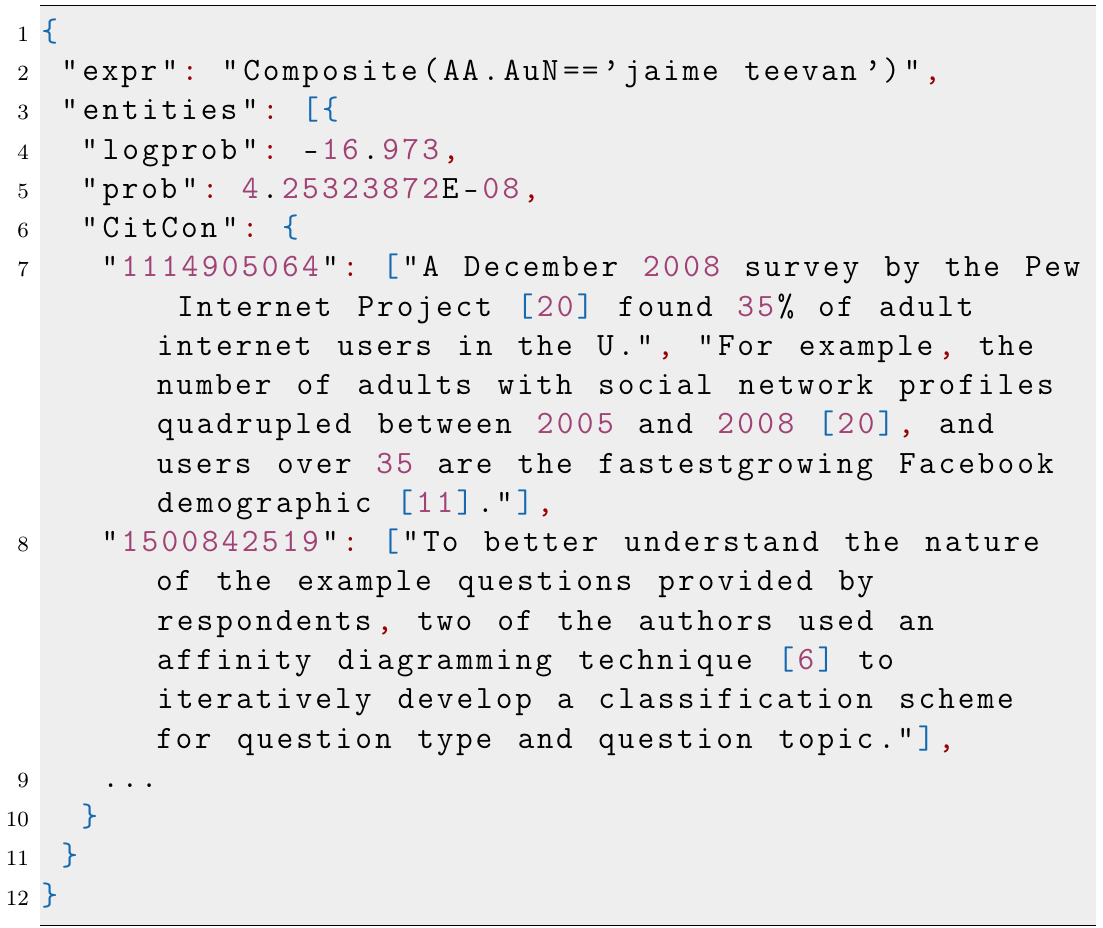
\includegraphics[width=12cm,keepaspectratio]{bilder/ResponseBeispiel}
	\caption{Response Beispiel}
	\label{fig:response-beispiel}
\end{figure}



Die Response aus Abbildung \ref{fig:response-beispiel} ist im JSON-Format. Diese dient genau wie XML für die Speicherung von menschlich lesbaren Daten.(vlg \cite{json}) Der gezeigte Ausdruck ist ein Beispiel, in dem nach einem Autor namens ’jaime teevan’ gesucht wird. Die Ausgabe der Attribute wurde nur auf ’CitCon’ beschränkt. Dies ist das Attribute für Zitate. Dennoch werden ’logprob’ und ’prob’ hinzugefügt. Da die Responses sehr kurz sein werden, müssen keine Parser selbst geschrieben werden. Somit kann ein fertiger Parser benutzen werden, der die Daten heraus filtert. Nun muss die Anfrage gesendet werden. 

Mit dieser relativ simplen API kommt aber auch eine Grenze. Es muss ein kostenloses Abonnement abgeschlossen werden, um Zugriff zu erhalten. Dafür ist ein an den Account gebundener Schlüssel nötig, mit dem die API benutzt werden kann. Im Monat dürfen mit diesem Schlüssel nur 10.000 Transaktionen getätigt werden. Durch diese Einschränkung werden hier nur selektive Beispiele präsentiert. Deshalb wird hier eine Funktion genutzt, die die ersten 200 Publikationen ausgibt. Mit diesen 200 Daten wird das Erweitern getestet und begutachtet.

Zunächst werden aus der Datenbank 200 Titel heraus genommen. Diese 200 Titel werden nun einzeln angepasst, um sie mit einer Request loszuschicken, denn die API kann keine Sonderzeichen oder Großschreibung verwenden. Nachdem die ganze Punktierung entfernt und kleingeschrieben wurde, wird die Anfrage mit der Bedingung geschickt, dass ‚Ti’ gleich des angepasstem Titel sein soll. ‚Ti’ steht für normalized title. Dieser Titel ist auch klein geschrieben und ohne Sonderzeichen. Damit werden schnell passende Publikationen gefunden. Mit der Filtereinstellung ‚CitCon’ kann nun die Id und der Abschnitt, der zitiert wurde, erhalten werden.



Nun wird eine Antwort erhalten wie in Abbildung \ref{fig:response-beispiel}. Daraufhin werden die wichtigen Informationen mit Hilfe eines Standard JSON-Parsers herausgefiltert. Falls der Titel kein Zitat besitzt, wird der Titel übersprungen und der nächste Titel angefragt. Wenn doch ein Zitat zu diesem Titel gefunden wurde, sind die relevanten Daten in der Antwort. Diese sind die Paper Id und das Zitat an sich. 

Die Paper Id ist in dieser Datenbank nicht zu gebrauchen, da diese nur zu den Publikationen in dem Microsoft Graphen gehören. Deswegen muss diese Id in etwas umwandeln werden, mit dem gearbeitet werden kann. In diesem Fall ist das wieder ein Titel. Für die Umwandlung wird eine weitere Anfrage an die Schnittstelle gestellt. Diese sucht nach Publikationen mit der selben ID, sodass der Titel zurückgegeben wird. Da die API nur Probleme bei der Eingabe von Sonderzeichen hat, aber nicht bei der Ausgabe,wird der Titel mit Sonderzeichen und Großschreibung zurückgegeben. Dazu wird der Filterwert  ‚DN’ verwendet, der den originalen Titel liefert. 

Somit sind alle Daten vorhanden, die gebraucht werden, um ein Zitat in die Datenbank einzuspeisen. Zunächst gibt es den Titel, wofür die Zitate gesucht wurden. Dann wurde ein das Zitat mit der Paper Id von der zitierten Publikation erhalten. Schlussendlich wurde daraus auch der Titel der Publikation erhalten. Nun muss nur noch der Titel in unserer Datenbank gefunden werden um die PublikationsId zu erhalten. Denn in unserer Relation, mit der die Zitierung dargestellt wird, werden die beiden Primärschlüssel der Publikationen benötigt. Es kann passieren das die Id von der Zitierten Publikation nicht in unserer Datenbank gefunden wird, da im Academic Graph mehr Werke gespeichert sind als in unserer und dadurch sich nicht alle Arbeiten überschneiden. Wurden die Daten gefunden, werden sie einfach mit einem DML-Befehl in die Datenbank eingefügt. 

So wird die Datenbank Schritt für Schritt erweitert. 





